\begin{figure}[h]
    \centering
    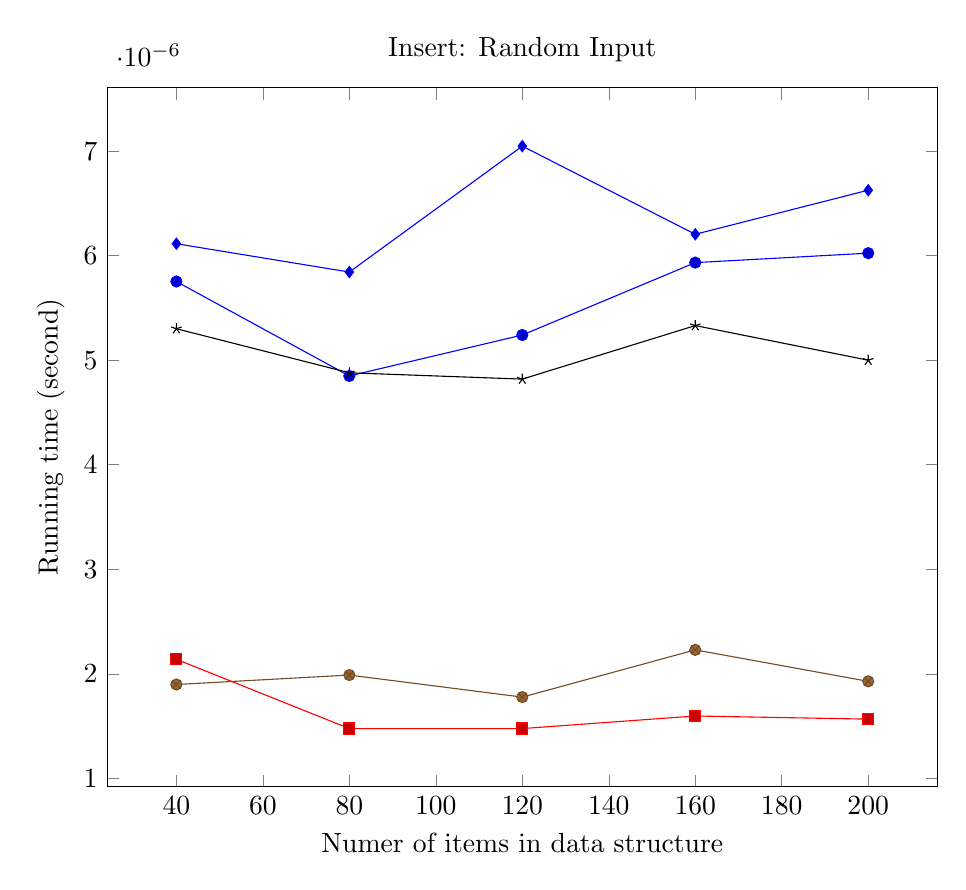
\begin{tikzpicture}
        \begin{axis}[
            xlabel={Numer of items in data structure},
            ylabel={Running time (second)},
            title={Insert: Random Input},
            width=\textwidth
        ]
		\addplot coordinates {
			(40, 5.752448932128118e-06)
			(80, 4.848922921496524e-06)
			(120, 5.240450859389511e-06)
			(160, 5.933154134041274e-06)
			(200, 6.023506735175488e-06)
		};
		\addplot coordinates {
			(40, 2.1383448910228252e-06)
			(80, 1.4757591500824673e-06)
			(120, 1.4757591500824673e-06)
			(160, 1.5962292845728143e-06)
			(200, 1.5661117508614098e-06)
		};
		\addplot coordinates {
			(40, 1.89740462168686e-06)
			(80, 1.987757222821074e-06)
			(120, 1.7769344868412418e-06)
			(160, 2.2286974918017678e-06)
			(200, 1.9275221553982645e-06)
		};
		\addplot coordinates {
			(40, 5.300685926812321e-06)
			(80, 4.879040455207928e-06)
			(120, 4.818805388140391e-06)
			(160, 5.330803460523726e-06)
			(200, 4.999510590053547e-06)
		};
		\addplot coordinates {
			(40, 6.11385933595443e-06)
			(80, 5.842801533262332e-06)
			(120, 7.047502879942158e-06)
			(160, 6.204211937088644e-06)
			(200, 6.6258574086930365e-06)
		};
        \legend{}
        \end{axis}
    \end{tikzpicture}
    \caption{Average of 0 operations, benchmarked every 0, starting at 0.}
\end{figure}